\documentclass[11pt,a4paper]{article}
\usepackage[T1]{fontenc}
\usepackage[utf8]{inputenc}
\usepackage{amsmath}
\usepackage{amssymb}
\usepackage{graphicx}
\usepackage[margin=2.5cm]{geometry}
\usepackage[hidelinks]{hyperref}

% Standalone draft of the performance chapter. The counters continue the
% numbering of the report, so that section, table, figure and equation
% numbers match the ones the chapter will carry once inserted.
\setcounter{section}{4}
\setcounter{table}{5}
\setcounter{figure}{27}
\setcounter{equation}{12}

\begin{document}

\section{Performance analysis}

\subsection{Sequential baseline}

The deterministic model above is also the reference problem for the
performance analysis of this chapter. Timings are taken in a separate
release build with visualisation and diagnostic output disabled, thread
counts pinned to one, and reported as the median of five runs after one
warm-up.

\begin{table}[htbp]
\centering
\begin{tabular}{rrrrr}
\hline
Elements per connection & Unknowns & Matrix nonzeros & 100 steps [s] & Per step [s] \\
\hline
1 & 83   & 2343  & 0.0832 & 0.00083 \\
2 & 1213 & 5733  & 1.8694 & 0.01869 \\
4 & 3473 & 12513 & 1.5486 & 0.01549 \\
8 & 7993 & 26073 & 2.2343 & 0.02234 \\
\hline
\end{tabular}
\caption{\footnotesize Sequential baseline for the deterministic model.
Assembly accounts for less than one percent of the total in every refined
case.}
\label{tab:seqbaseline}
\end{table}

Two facts emerge from Table~\ref{tab:seqbaseline} and they set the agenda
for what follows. First, in every refined case more than 99\% of the time
is spent in the time loop (95.9\% at one element per connection) and almost
none in assembly or input, so the target for optimisation is the repeated
sparse factorisation forced by the semi-implicit scheme (Table 5), not the
finite element assembly. Second, the cost per step is not a function of the
number of unknowns alone: the two-element mesh, with 1213 unknowns, costs
more than the four-element mesh with 3473. The two-element mesh inherits a
hub-dominated sparsity pattern from the connectome, and sparse
factorisation depends on the elimination ordering and the resulting fill-in
at least as much as on the matrix dimension.

For scale, [9] report that their nodal model runs its 100 implicit steps in
0.55~s without output on a standard laptop; our metric-graph formulation at
the same 83 unknowns takes 0.083~s for its 100 semi-implicit steps. The
machines and the schemes differ, so this is an order-of-magnitude check
rather than a comparison, but it confirms that the P1 metric-graph
formulation carries no cost penalty over the nodal network model at the
coarsest mesh, while allowing arbitrary refinement inside the connections.

\begin{figure}[htbp]
\centering
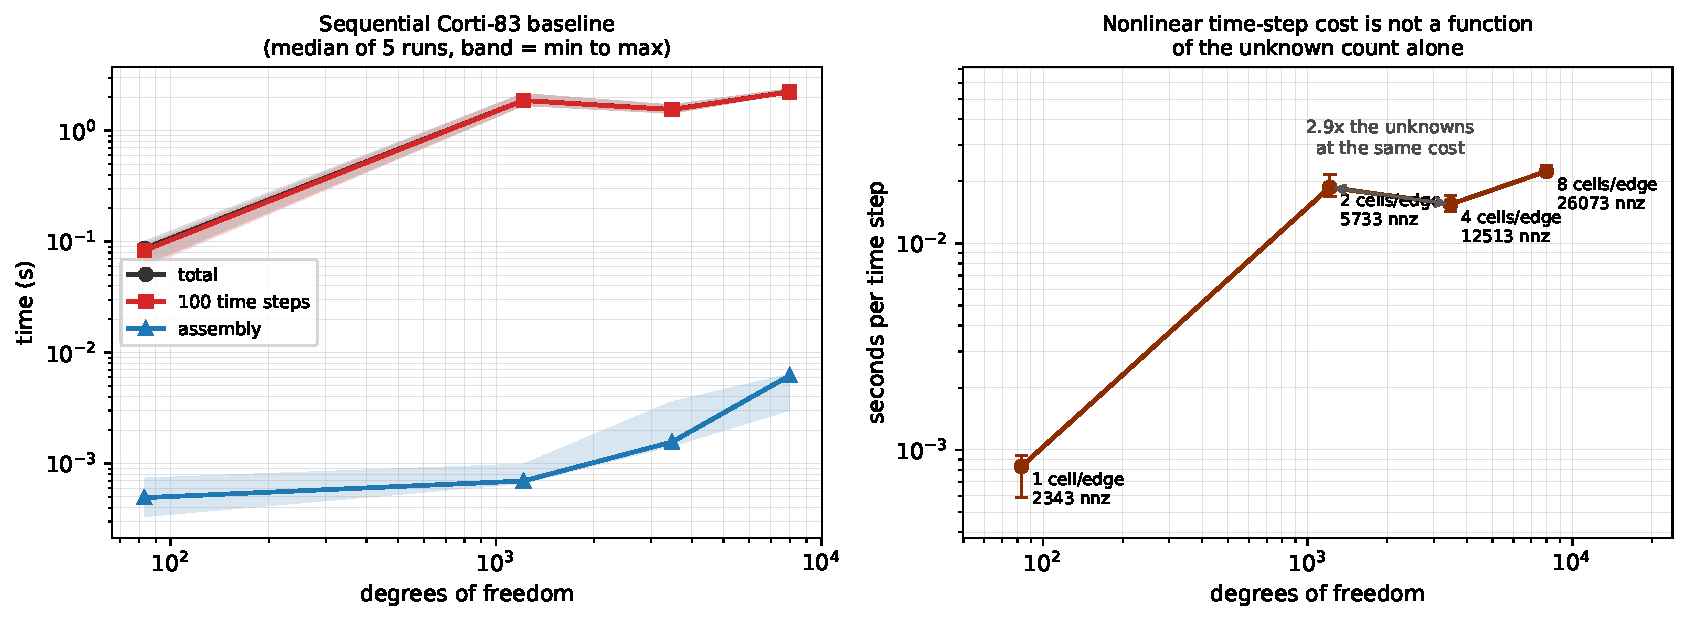
\includegraphics[width=\textwidth]{../benchmarks/22_fisher_kolmogorov_sequential_performance/results/sequential_performance.pdf}
\caption{\footnotesize Sequential baseline. (a) assembly, time loop and
total against the number of unknowns, with the band spanning the minimum
and maximum of five runs; the total is hidden by the time loop, which
accounts for 95.9\% of it on the coarsest mesh and for more than 99\% on
the refined ones, so the two curves overlap. (b) cost per time step,
showing that it is not a function of the unknown count alone: the
two-element mesh costs more per step than the four-element one.}
\label{fig:seqbaseline}
\end{figure}

This is precisely the observation that motivates the reordering study of
the next section, where bandwidth, profile, factor fill and factorisation
time are measured for different orderings before any parallel scaling
result is interpreted.

\subsection{Matrix ordering and the sequential solver}
\label{sec:ordering}

With the semi-implicit scheme of Table 5 every time step advances the
concentration by solving one linear system. Writing $M$ for the mass
matrix, $H$ for the discrete Hamiltonian of Section 2.2 and $W(v)$ for the
reaction matrix assembled with the weight $\alpha(1-v)$, the
Crank--Nicolson update with the second-order extrapolation
$\hat c^{\,n+1} = \tfrac{3}{2} c^{n} - \tfrac{1}{2} c^{n-1}$ reads
\begin{equation}
K^{n} c^{n+1} = b^{n},
\qquad
K^{n} = M + \tfrac{\Delta t}{2} H - \tfrac{\Delta t}{2} W(\hat c^{\,n+1}),
\label{eq:stepmatrix}
\end{equation}
with $b^{n} = \bigl(M - \tfrac{\Delta t}{2} H + \tfrac{\Delta t}{2}
W(\hat c^{\,n+1})\bigr) c^{n}$. The sparsity pattern of $K^{n}$ is that of
$M + H$ and never changes; its values change at every step through the
extrapolated reaction weight, so the solver must refactorise at every step.
All three matrices are symmetric, hence so is $K^{n}$. The solver used in
the preceding chapters treats the system with the sparse LU factorisation
of Eigen and its default fill-reducing column ordering, COLAMD, recomputing
the factorisation from scratch at each step. This section asks whether that
factorisation, which Table~\ref{tab:seqbaseline} identifies as the dominant
cost, is performed in the right ordering.

To compare orderings under the exact conditions of the production run we
replay the same time loop, with the same matrices and right-hand sides, and
hand the matrix of every step to one of six variants: the production LU
with COLAMD, LU on the natural ordering, LU with the approximate minimum
degree ordering AMD, LU on a reverse Cuthill--McKee (RCM)
permutation of the matrix and, exploiting symmetry, the $LDL^{T}$
factorisation on the AMD and on the natural ordering. Over one hundred
steps the trajectories of all variants agree with the production one to
within $4\times10^{-14}$ in the maximum norm, so the comparison is between
numerically equivalent solvers. For each variant we record the bandwidth
and profile of the matrix handed to the solver, the number of nonzeros of
its factors and the per-step cost split into the rebuild of the matrix, the
factorisation and the triangular solves.

The natural ordering is not an arbitrary baseline, because the assembly
numbers the unknowns in a specific way: the interior unknowns of each
connection are numbered consecutively, connection after connection, and the
83 vertex unknowns come last. In this numbering $K^{n}$ is an arrow matrix,
a block-diagonal part with one tridiagonal block per connection bordered by
the rows and columns of the vertices. Gaussian elimination in natural order
eliminates the interiors of each connection inside their own tridiagonal
block and produces new nonzeros only in the border, so the fill-in is
essentially confined to an $83\times 83$ block regardless of refinement.

\begin{table}[htbp]
\centering
\footnotesize
\begin{tabular}{lrrrrrr}
\hline
& \multicolumn{2}{c}{2 elements, $n=1213$}
& \multicolumn{2}{c}{8 elements, $n=7993$}
& \multicolumn{2}{c}{64 elements, $n=71273$} \\
Ordering & factor nonzeros & step [ms] & factor nonzeros & step [ms]
& factor nonzeros & step [ms] \\
\hline
LU, COLAMD      & 182208 & 26.84 & 104934  & 21.16  & 484614   & 140.31 \\
LU, natural     & 10522  & 2.35  & 51202   & 10.43  & 430882   & 81.38  \\
LU, RCM         & 80570  & 8.13  & 1103850 & 162.93 & 11594218 & 2013.1 \\
LDLT, natural   & 5261   & 0.61  & 25601   & 1.93   & 215441   & 21.04  \\
\hline
\end{tabular}
\caption{\footnotesize Ordering study on the connectome meshes with 2, 8
and 64 elements per connection: nonzeros of the computed factors and median
per-step cost (matrix rebuild, factorisation and triangular solves) over
100 steps of the semi-implicit scheme. RCM is applied as an explicit
symmetric permutation of the matrix; the other variants reorder internally.}
\label{tab:ordering}
\end{table}

Table~\ref{tab:ordering} and Figure~\ref{fig:ordering} collect the results.
Three observations follow. First, the production ordering is responsible
for the anomaly of Table~\ref{tab:seqbaseline}: on the two-element mesh
COLAMD produces 182208 factor nonzeros, more than the 77828 it produces on
the four-element mesh, so the smaller problem really is more expensive to
factorise. The anomaly is a property of the ordering heuristic on this
hub-dominated pattern, not of the problem. Second, minimising bandwidth is
the wrong objective for this structure. RCM reduces the bandwidth from 7989
to 937 on the eight-element mesh, but it destroys the arrow structure: at
64 elements per connection its profile is eleven times that of the natural
ordering and its factors carry 27 times the nonzeros, for a step of about
two seconds. Third, the natural ordering is already close to fill-optimal,
below COLAMD on every refined mesh, and the symmetric $LDL^{T}$
factorisation on the natural ordering halves the remaining work: at 64
elements per connection it stores 215441 factor nonzeros against the 484614
of the production configuration and completes a step in 21.0~ms against
140.3~ms, a factor of 6.7. AMD paired with $LDL^{T}$ finds essentially the
same fill, 214939 nonzeros, but repeats its ordering analysis at every
rebuild and ends up nearly twice as slow, so the natural ordering obtains
the same quality at no cost.

\begin{figure}[htbp]
\centering

\includegraphics[width=\textwidth]{performance_ordering.pdf}
\caption{\footnotesize The ordering study. (a) factor nonzeros against the
number of unknowns for the four orderings of Table~\ref{tab:ordering}; the
marked point is the two-element mesh, on which the production ordering
fills more than on the next two meshes. (b) median cost per time step. The
$LDL^{T}$ factorisation on the natural ordering is the sequential reference
adopted for the rest of the chapter.}
\label{fig:ordering}
\end{figure}

We therefore adopt the $LDL^{T}$ factorisation on the natural ordering as
the sequential reference. This is an algorithmic improvement, obtained with
the same discretisation and the same arithmetic. It also moves the
bottleneck: at 64 elements per connection the factorisation now costs
6.1~ms and the triangular solves 0.9~ms, while rebuilding the sparse matrix
costs 14.0~ms per step. Once the ordering is right, most of the step is
spent assembling a global matrix whose structure repeats, connection by
connection, a pattern that the factorisation then eliminates. The next
section removes the global matrix altogether.

\subsection{Static condensation}
\label{sec:condensation}

The arrow structure can be exploited before any global factorisation is
performed. Let $E$ collect the interior unknowns of the connections and $V$
the 83 vertex unknowns; splitting the system of
Eq.~\eqref{eq:stepmatrix} accordingly gives
\begin{equation}
\begin{pmatrix} K_{EE} & K_{EV} \\ K_{VE} & K_{VV} \end{pmatrix}
\begin{pmatrix} c_{E} \\ c_{V} \end{pmatrix}
=
\begin{pmatrix} b_{E} \\ b_{V} \end{pmatrix},
\qquad K_{EV} = K_{VE}^{\top},
\label{eq:blocks}
\end{equation}
where $K_{EE}$ is block diagonal with one tridiagonal block per connection,
because interior nodes couple only to their neighbours on the same
connection. Eliminating $c_{E}$ exactly gives the Schur complement system
on the vertices,
\begin{equation}
S \, c_{V} = g,
\qquad
S = K_{VV} - K_{VE} K_{EE}^{-1} K_{EV},
\qquad
g = b_{V} - K_{VE} K_{EE}^{-1} b_{E},
\label{eq:schur}
\end{equation}
followed by the back substitution
$c_{E} = K_{EE}^{-1} \bigl(b_{E} - K_{EV} c_{V}\bigr)$. No approximation is
involved: the pair $(c_{E}, c_{V})$ solves Eq.~\eqref{eq:stepmatrix}
exactly, and the reduction is Gaussian elimination in the natural ordering,
written so that the elimination of each connection becomes an independent
task.

The per-connection work is small and structured. A connection with $m$
elements contributes a tridiagonal $(m-1)\times(m-1)$ block of $K_{EE}$,
two coupling columns towards its endpoints and the interior part of the
right-hand side; the entries are the same element integrals as in the
production assembly, evaluated with the extrapolated reaction weight of the
current step. The Thomas algorithm factorises the tridiagonal block in
$O(m)$ operations, and sweeps against the right-hand side and the two
coupling columns produce the $2\times 2$ contribution of the connection to
$S$, its two entries of $g$ and the vectors reused by the back
substitution. The interface matrix $S$ is $83\times 83$ with the sparsity
of the connectome plus the diagonal; we store it as a dense matrix and
factorise it by a dense $LDL^{T}$ at every step, a constant cost of about
0.1~ms independent of refinement. The global sparse matrix of
Eq.~\eqref{eq:stepmatrix} is never assembled.

For the timing study the connectome mesh is refined up to 128 elements per
connection, that is 143593 unknowns. The topology is kept fixed and only
the finite-element resolution along each connection is increased, providing
a controlled increase in the number of unknowns without modifying the
underlying connectome.

\begin{table}[htbp]
\centering
\begin{tabular}{rrrrr}
\hline
Elements per connection & Unknowns & Full system [ms] & Condensed [ms] & Ratio \\
\hline
8   & 7993   & 3.61  & 1.03  & 3.5 \\
16  & 17033  & 8.34  & 1.99  & 4.2 \\
32  & 35113  & 13.52 & 4.11  & 3.3 \\
64  & 71273  & 35.02 & 6.73  & 5.2 \\
128 & 143593 & 64.45 & 10.99 & 5.9 \\
\hline
\end{tabular}
\caption{\footnotesize Static condensation against the full-system
$LDL^{T}$ factorisation on the natural ordering: median per-step cost over
100 steps. The two solvers advance the same trajectory back to back in the
same process, so each ratio compares two measurements of the same run.}
\label{tab:condensation}
\end{table}

Table~\ref{tab:condensation} compares the condensed step with the
full-system $LDL^{T}$ reference of Section~\ref{sec:ordering}; the two
solvers run back to back in the same process, so each ratio compares two
measurements of the same run, and the absolute times differ from those of
Table~\ref{tab:ordering} by the run-to-run variability of the machine. The
condensed step is between 3.5 and 5.9 times faster than the full-system
one, with the largest gain on the finest mesh, and its cost grows roughly
linearly with the number of unknowns. Figure~\ref{fig:condensation}(b)
shows where the time goes: at 128 elements per connection the
per-connection elimination takes 10.56~ms, the back substitution 0.34~ms
and the interface solve 0.09~ms, less than one percent of the step. Almost
the entire step is independent work on the connections, which is the
property the parallel versions of the next section exploit.

\begin{figure}[htbp]
\centering

\includegraphics[width=\textwidth]{performance_condensation.pdf}
\caption{\footnotesize Static condensation. (a) median per-step cost of the
condensed solver against the full-system reference, with the ratio at the
finest mesh. (b) phase split of the condensed step: the interface solve is
constant across refinement and the step is dominated by the independent
per-connection eliminations.}
\label{fig:condensation}
\end{figure}

The condensed trajectory was compared step by step with the production
solver over one hundred steps on the meshes up to eight elements per
connection, with maximum differences of about $10^{-14}$, and against the
full-system $LDL^{T}$ solver on the finer meshes, with differences below
$3\times10^{-14}$: static condensation is the same computation reorganised.
Taking the two experiments together, the per-step cost at 64 elements per
connection falls from the 140.3~ms of the production configuration to
6.73~ms, a factor of about twenty from ordering, symmetry and condensation
combined. This is an algorithmic gain, measured with one thread; we keep it
separate from the parallel speedups of Section~\ref{sec:scaling}, which are
measured against the condensed solver itself.

\subsection{Parallel implementation}
\label{sec:parallel}

Both parallel versions parallelise the condensed step. The natural unit of
work is the connection: its elimination and its back substitution touch
only its own interior storage and contribute to the interface system
through a $2\times 2$ block and two right-hand-side entries. The interface
solve stays serial in the OpenMP version and replicated in the MPI version,
a choice justified by its constant cost of about 0.1~ms.

\subsubsection{OpenMP}

The elimination loop and the back-substitution loop over the connections
are shared among the threads. Each connection writes to its own slice of
the preallocated work arrays, so the loops need no synchronisation; the
contributions to $S$ and $g$ are accumulated in thread-private storage and
merged once per thread at the end of the elimination loop. A single thread
then factorises the interface system and the back substitution runs again
in parallel. The arithmetic is identical to the sequential condensed step
except for the order in which the per-thread contributions are summed into
the interface system, so the two versions agree to round-off: advancing
both engines in lockstep and comparing every step gives maximum differences
below $3\times10^{-14}$ on the eight-element mesh with two, four and eight
threads and on the 128-element mesh with eight threads.

\subsubsection{MPI}

The connections are assigned to the ranks in contiguous blocks, sized so
that every rank owns nearly the same number of interior unknowns. Each rank
stores the replicated vertex states and the interiors of its own
connections only, eliminates its connections and accumulates its local
contribution to the interface system. One reduction phase per step, two
\texttt{MPI\_Allreduce} calls that sum the $83\times 83$ interface matrix
and its right-hand side across the ranks, carries a fixed payload of about
55~kB independent of refinement; every rank then factorises the interface system
redundantly, which at this size is cheaper than distributing the
factorisation, and back-substitutes its own connections without further
communication. Per-step communication is therefore constant while the
distributed work grows with the mesh. The same lockstep comparison against
the sequential condensed solver, gathering the distributed state at every
step, gives maximum differences below $10^{-14}$ on the eight-element mesh
with two, four and eight ranks and on the 128-element mesh with eight
ranks.

A hybrid variant is obtained by compiling the MPI version with OpenMP
enabled, so that each rank runs its elimination and back-substitution loops
with threads and ranks and threads can be traded at a fixed number of
workers. Its lockstep differences are at the same level.

\subsection{Parallel performance}
\label{sec:scaling}

All scaling experiments run on the mesh with 128 elements per connection
and 143593 unknowns, chosen because the coarser meshes complete a condensed
step in a few milliseconds at most, leaving little work to distribute. The
machine is the same laptop as before, with four physical cores and two
hardware threads per core (simultaneous multithreading, SMT); up to four
workers each worker is bound to its own physical core and eight workers use
the hardware threads. Every configuration advances 200 steps and every
reported time is the median over the steps and over three repeated runs.
Each experiment measures its own sequential reference in its own session;
the references are 9.58, 8.07 and 8.40~ms per step for the OpenMP, MPI and
hybrid experiments, a spread that reflects the run-to-run variability of
the machine, and every speedup is computed against the reference of its own
experiment.

\begin{table}[htbp]
\centering
\begin{tabular}{lrrr}
\hline
Threads & Per step [ms] & Speedup & Efficiency \\
\hline
sequential & 9.58 & --   & --   \\
2          & 5.65 & 1.69 & 0.85 \\
4          & 3.37 & 2.84 & 0.71 \\
8          & 2.06 & 4.64 & 0.58 \\
\hline
\end{tabular}
\caption{\footnotesize OpenMP strong scaling of the condensed step on the
mesh with 128 elements per connection: medians over 200 steps and three
runs, speedups against the sequential condensed reference of the same
experiment.}
\label{tab:openmp}
\end{table}

Table~\ref{tab:openmp} reports the OpenMP scaling. Running the OpenMP build
on a single thread costs 10.70~ms against the 9.58~ms reference, an
overhead of about twelve percent for the threaded code path. From there the
scaling is regular: 1.69 at two threads, 2.84 at four and 4.64 at eight.
The four-thread configuration is the clean measurement of the physical
machine, one thread per core, with a parallel efficiency of 0.71; at eight
threads the step still shortens, from 3.37 to 2.06~ms, but each core now
runs two hardware threads. The lower efficiency at eight threads is
consistent with the use of SMT on a four-core processor and with the
increasing relative cost of serial and memory-bound phases. The phase split
at eight threads confirms the picture: the two parallel loops account for
1.92~ms of the 2.06~ms step, while the merge of the thread contributions
and the serial interface solve account for the remaining 0.14~ms.

\begin{table}[htbp]
\centering
\begin{tabular}{lrrrr}
\hline
Ranks & Per step [ms] & Reduction [ms] & Speedup & Efficiency \\
\hline
sequential & 8.07 & --   & --   & --   \\
2          & 4.66 & 0.09 & 1.73 & 0.87 \\
4          & 4.29 & 0.71 & 1.88 & 0.47 \\
8          & 2.56 & 0.20 & 3.15 & 0.39 \\
\hline
\end{tabular}
\caption{\footnotesize MPI strong scaling of the condensed step on the same
mesh: medians over 200 steps and three runs. The reduction column is the
median per-step cost of summing the interface system across the ranks
(\texttt{MPI\_Allreduce}).}
\label{tab:mpi}
\end{table}

Table~\ref{tab:mpi} reports the MPI scaling. The single-rank run costs
8.93~ms against the 8.07~ms reference, an overhead of about eleven percent.
Two ranks reach a speedup of 1.73, in line with the OpenMP result, but four
ranks reach only 1.88: the median cost of the reduction grows to 0.71~ms
and, since the reduction synchronises the ranks, it absorbs as waiting time
any imbalance in the moment at which the ranks finish their elimination;
the payload itself does not change. At eight ranks the reduction falls back
to 0.20~ms and the speedup reaches 3.15. At every worker count the MPI
version is slower than the OpenMP one on this machine, which is the
expected outcome on a single shared-memory node: the MPI version pays the
message and synchronisation costs and replicates the interface solve on
every rank, without the shared address space that makes the threaded
version cheap. These runs say nothing about distributed memory, where MPI
is the only option of the two; we have not run the code on more than one
node and draw no conclusion beyond one.

\begin{figure}[htbp]
\centering

\includegraphics[width=\textwidth]{performance_scaling.pdf}
\caption{\footnotesize Parallel performance on the mesh with 128 elements
per connection. (a) strong scaling of the OpenMP and MPI versions; each
series is normalised by the sequential condensed reference of its own
experiment (9.58 and 8.07~ms per step). The one-worker configurations,
omitted from the curves, cost 10.70 and 8.93~ms. (b) the four arrangements
of eight workers with the hybrid build, as MPI ranks $\times$ OpenMP
threads, with speedups against the reference of the hybrid experiment
(8.40~ms per step).}
\label{fig:scaling}
\end{figure}

Figure~\ref{fig:scaling}(b) compares the four ways of arranging eight
workers with the hybrid build, from one rank with eight threads to eight
ranks with one thread each. The step time degrades monotonically as workers
shift from threads to ranks, from 2.06 to 2.61~ms, and the two ends
reproduce the pure OpenMP and pure MPI measurements within the variability
across sessions; the reduction cost grows with the number of ranks, from
essentially zero to 0.21~ms. On one node, at a fixed number of workers,
threads are preferable to ranks and the hybrid arrangements sit in between.

Combining the algorithmic and the parallel gains, and comparing
measurements from different sessions, the cost of a time step on the
128-element mesh falls from 64.5~ms for the best full-system factorisation
to 2.06~ms for the condensed solver on eight threads, a combined factor of
about thirty; the condensation contributes a factor of 5.9 and the
parallelisation the rest. The performance study thus closes the chain
opened by Table~\ref{tab:seqbaseline}. The anomaly of the sequential
baseline was an ordering artefact and the natural ordering with a symmetric
factorisation removes it; static condensation turns the arrow structure of
the connectome discretisation into independent per-connection work with a
constant-cost interface; OpenMP converts that structure into a speedup of
2.84 on the four physical cores and 4.64 with SMT; the MPI version is
correct and scales, but on a single node it does not match the threaded
version and its value lies in distributed settings we have not measured.
Every parallel configuration reproduces the sequential trajectory to
round-off, so all of the above is a reorganisation of the same computation.

\end{document}
